\section{Graphical User Interface}
This section presents and explains the wireframes of the application. These wireframes provide a visual overview of the layout and user interface design across various parts of the system, highlighting how users will interact with the application. Each wireframe corresponds to a specific microfrontend or the Application Shell and illustrates its core functionalities and structural components.

\subsubsection*{Application Shell}
\begin{figure}[h]
    \centerline{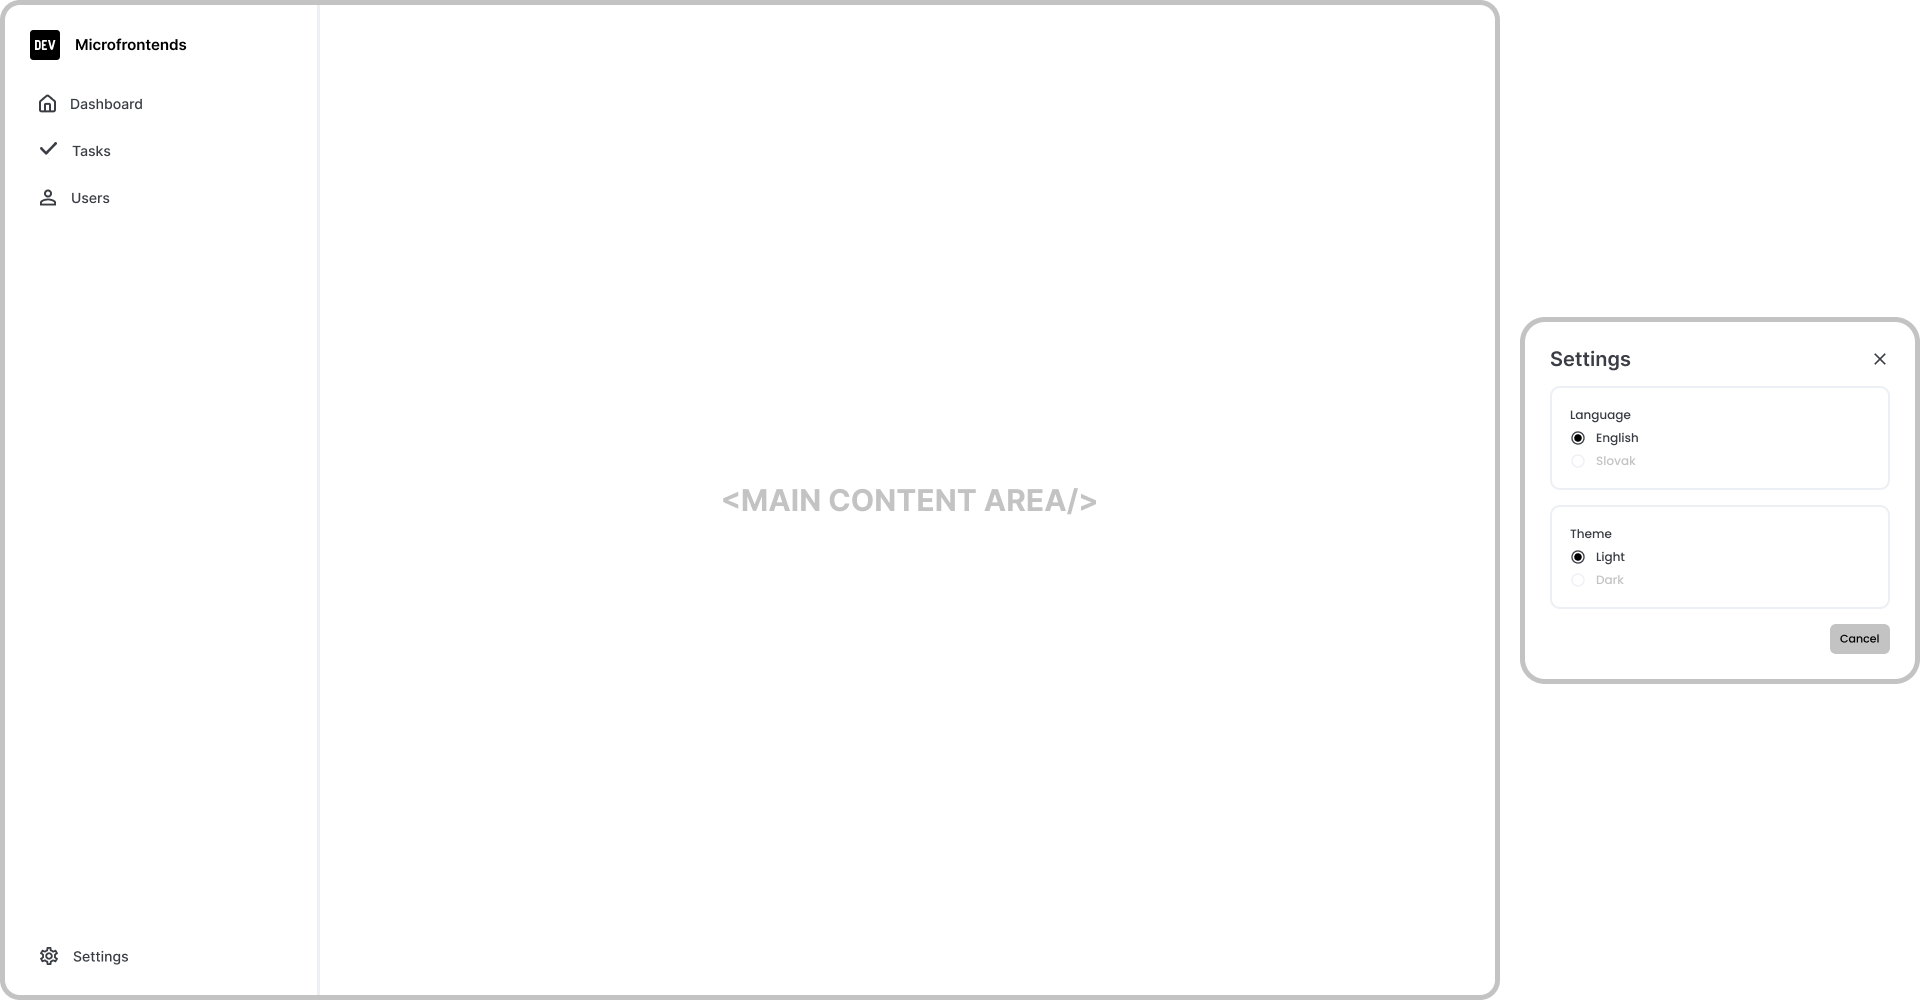
\includegraphics[width=1\textwidth]{images/wireframes/application-shell.png}}
    \caption[Application Shell wireframe]{Wireframe of the Application Shell interface}
    \label{fig:shell-wireframe} 
\end{figure}
As illustrated in Figure \ref{fig:shell-wireframe}, the Application Shell features a side panel that includes the application logo and navigation links for accessing each microfrontend, as well as the dashboard page. A settings button is located at the bottom of the side panel; when clicked, it opens a modal containing radio buttons for toggling the application's language (English/Slovak) and theme (light/dark). The main content area, positioned adjacent to the side panel, dynamically renders the active page—either a single microfrontend or the composed dashboard view.

\subsubsection*{User Microfrontend}
\begin{figure}[h]
\centerline{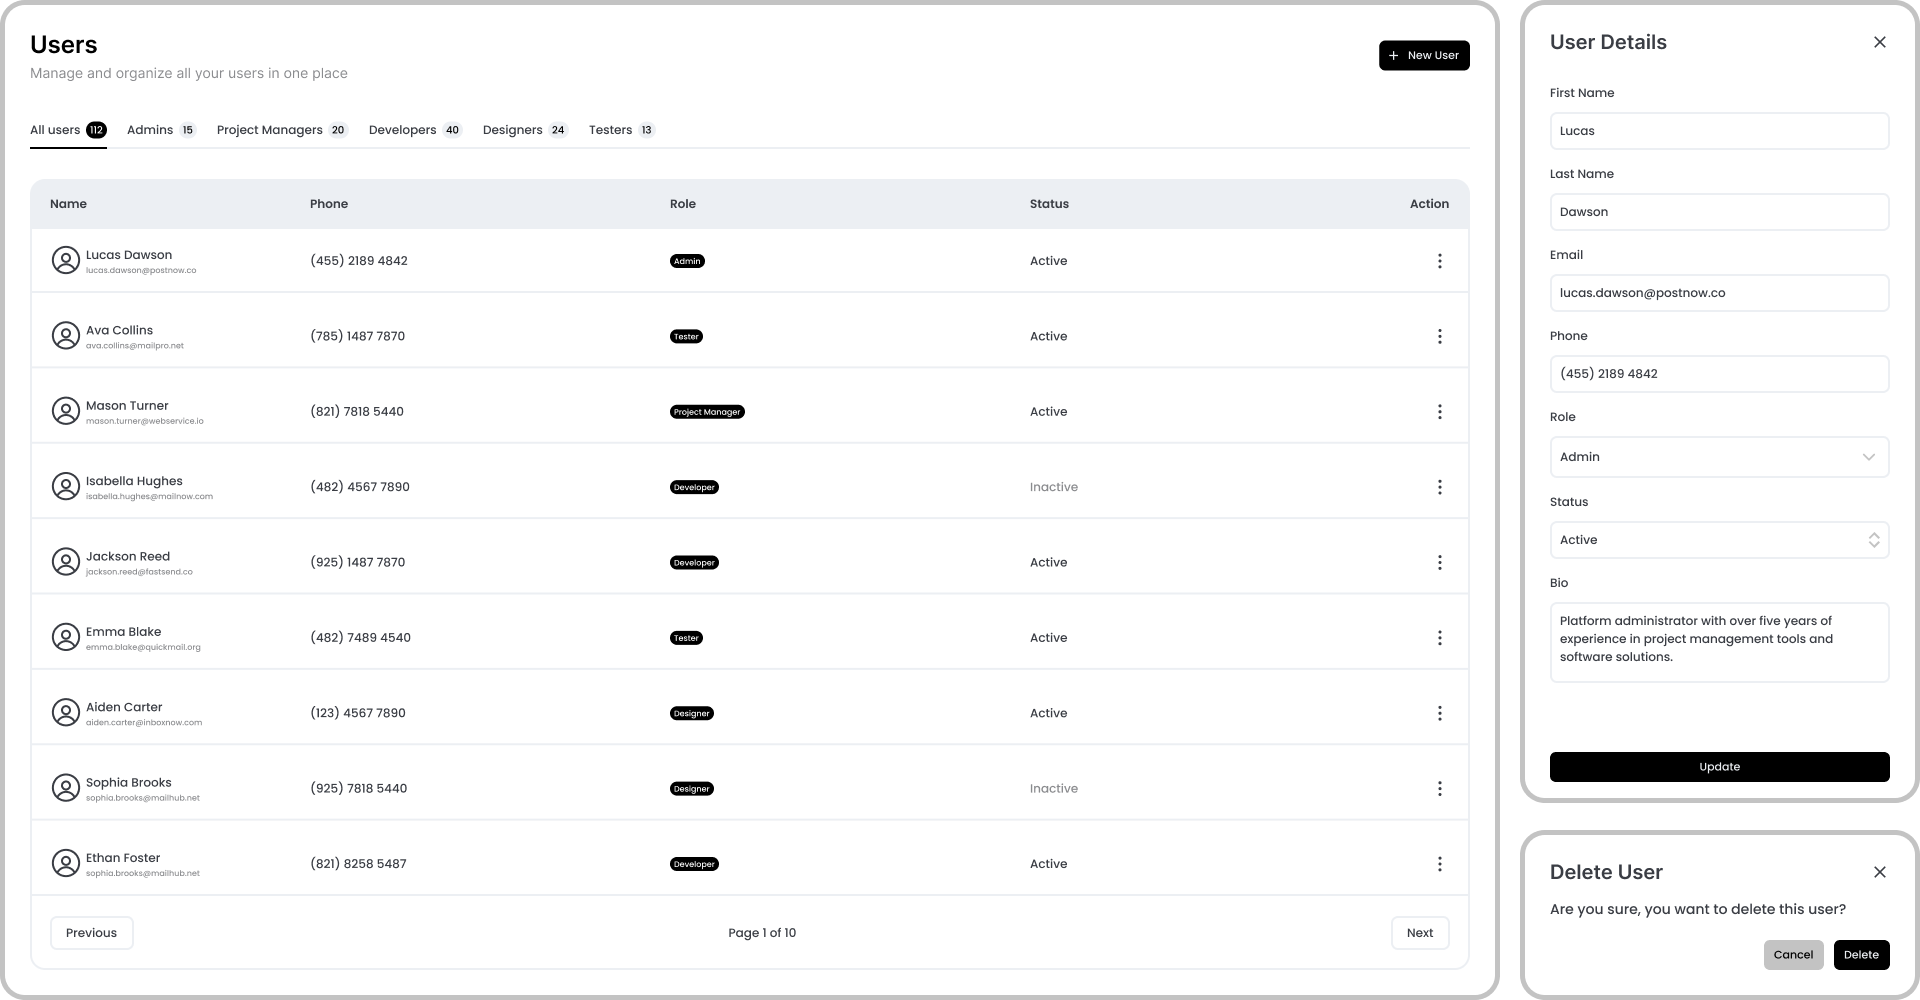
\includegraphics[width=1\textwidth]{images/wireframes/user-microfrontend.png}}
\caption[User Microfrontend wireframe]{Wireframe of the User Microfrontend interface}
\label{fig:user-wireframe}
\end{figure}
As illustrated in Figure \ref{fig:user-wireframe}, the User Microfrontend interface features a table in which each row represents a user. Key user details such as name, email, phone number, role, and status are displayed in respective columns. The final column contains an action button that opens a dropdown menu with options to view, edit, or delete the user. Upon selecting any of these actions, a modal window is triggered to perform the desired operation.

Above the table, a set of filter tabs allows users to quickly view subsets of users based on predefined roles (admins, project managers, developers, designers and testers). At the very top of the page is a top bar, which includes the page title, a subtitle, and a button labeled ``Add User''. Clicking this button opens a modal window for creating a new user.

\subsubsection*{Task Microfrontend}
\begin{figure}[h]
    \centerline{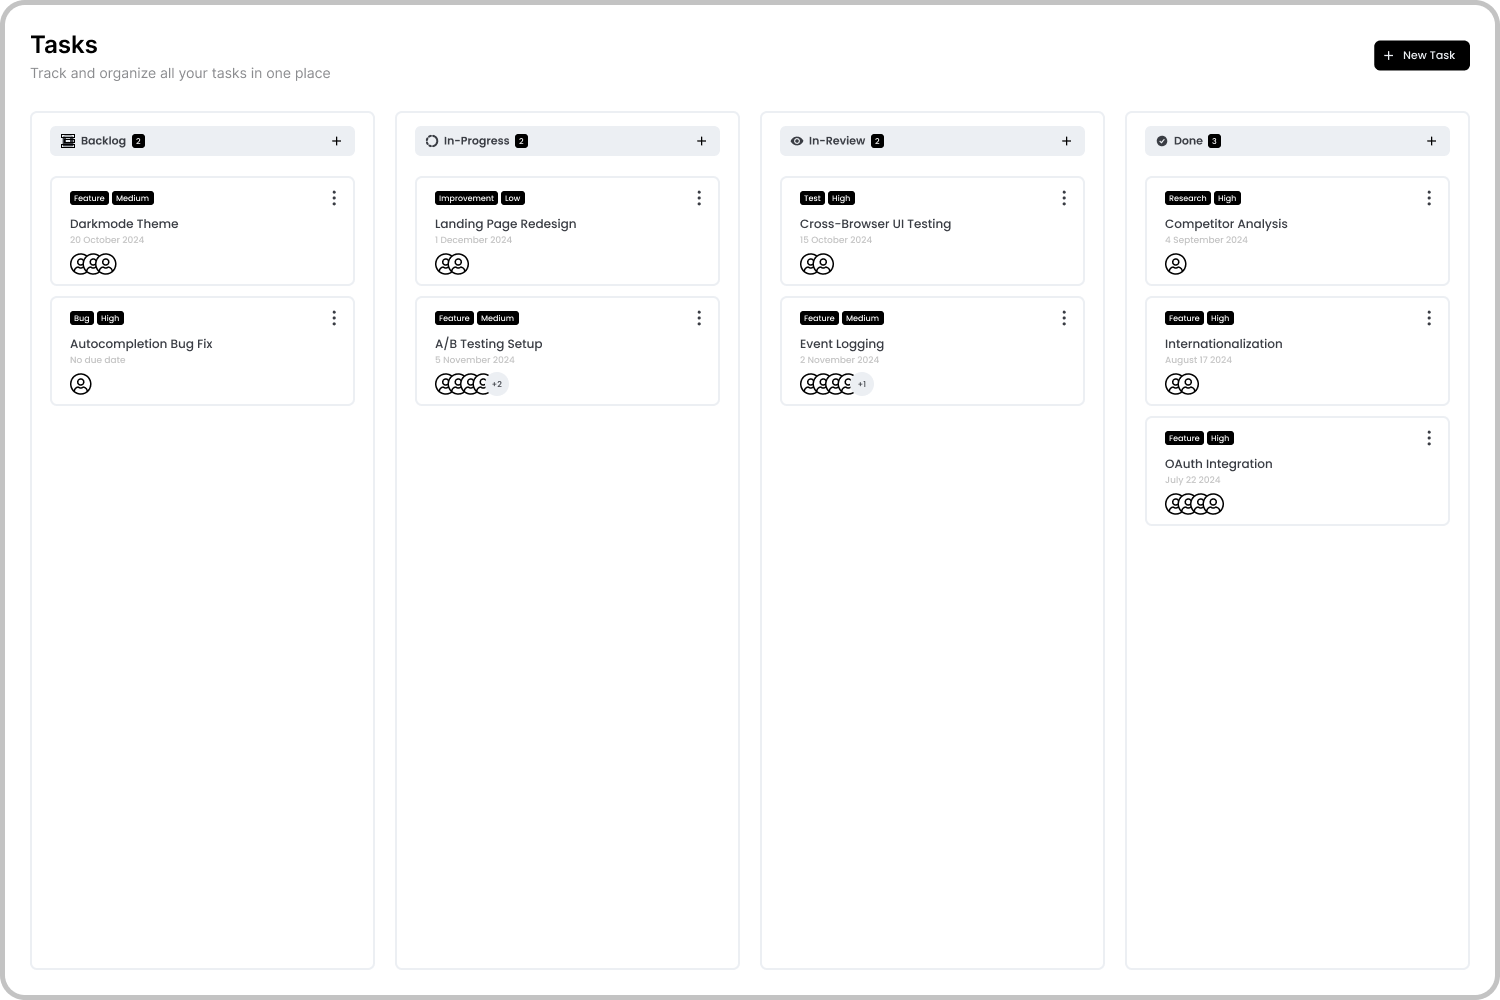
\includegraphics[width=1\textwidth]{images/wireframes/task-microfrontend.png}}
    \caption[Task Microfrontend wireframe]{Wireframe of the Task Microfrontend interface}
    \label{fig:task-wireframe}
\end{figure}
Figure \ref{fig:task-wireframe} illustrates the Task Microfrontend, which centers around a Kanban board. This board categorizes tasks into distinct stages such as \textit{Backlog}, \textit{In-Progress}, \textit{In-Review}, and \textit{Done}. Each task is visualized as a card that displays key metadata including the title, tag, assignees, and more. A three-dot menu in the top-right corner of each card allows users to view, edit, or delete the task via modal dialogs.

Each stage column features a button for creating tasks directly within that category. At the top of the interface is a top bar containing the page title, a subtitle, and a ``New Tas'' button that opens a dedicated modal for task creation.

\subsubsection*{Dashboard}
\begin{figure}[h]
    \centerline{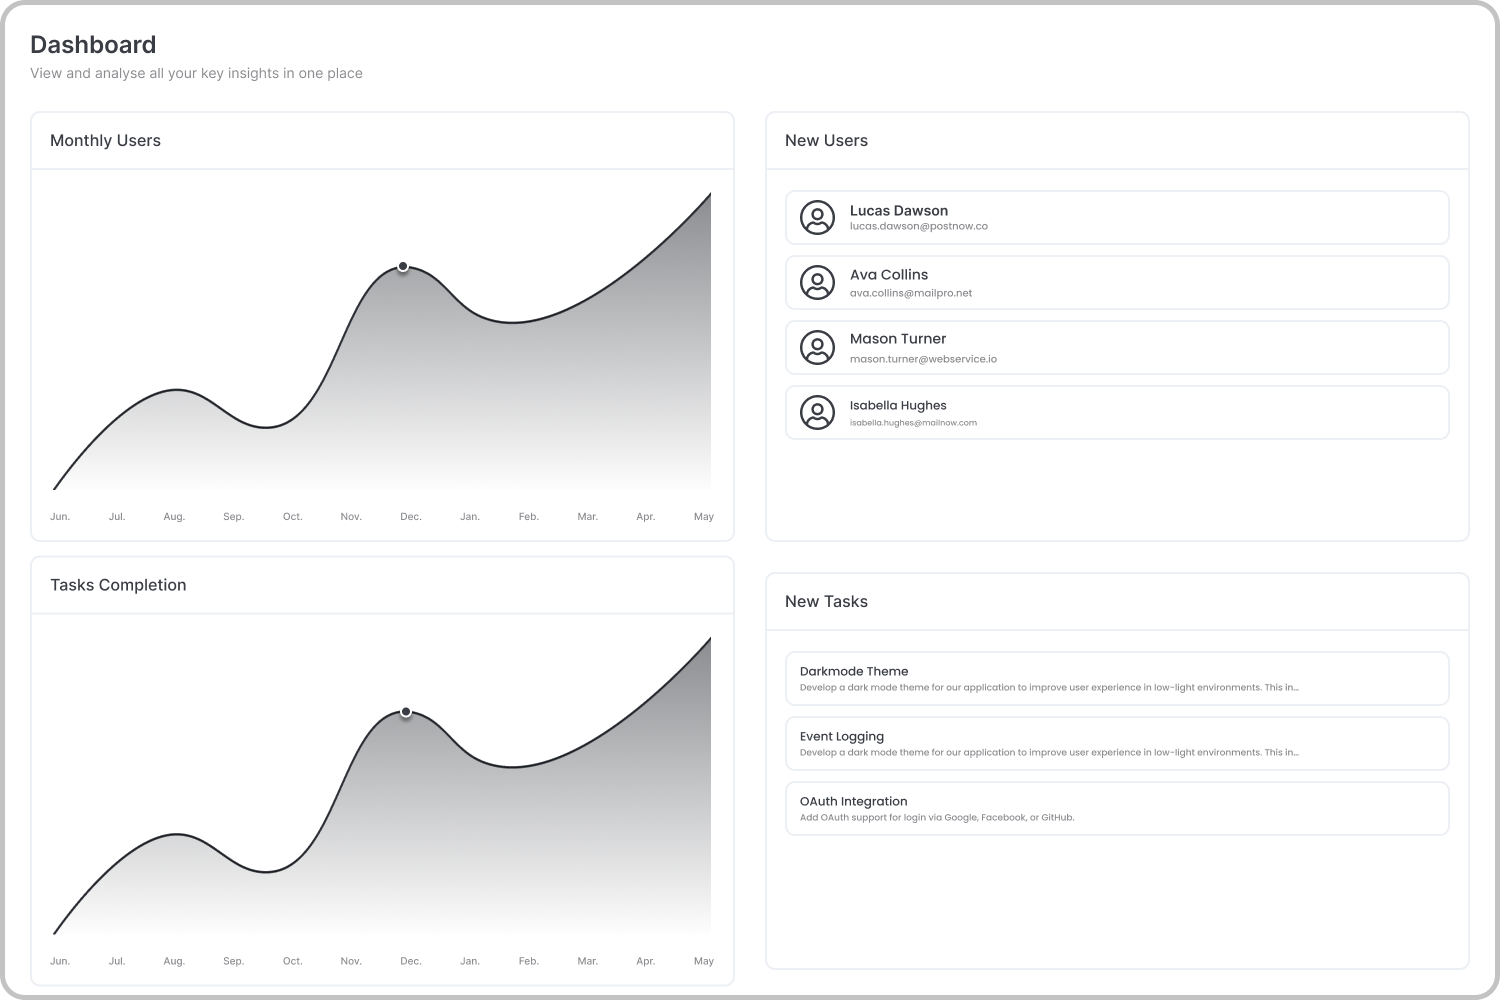
\includegraphics[width=1\textwidth]{images/wireframes/dashboard.png}}
    \caption[Dashboard wireframe]{Wireframe of the Dashboard interface}
    \label{fig:dashboard-wireframe}
\end{figure}
Figure \ref{fig:dashboard-wireframe} shows the Dashboard, which combines the User and Task Microfrontends in compact modes, along with components from the Application Shell. Positioned at the top of the layout is the global top bar, rendered by the Application Shell. Below the top bar, the Task Microfrontend displays the monthly task count graph and a widget listing new tasks. The lower portion of the dashboard features the User Microfrontend, which displays a monthly user count graph and a widget for new users. These microfrontends are rendered in compact mode and interact with each other as discussed in the section \ref{sec:SystemArchitecture}.
